\documentclass[
  a4paper,            % DIN A4
  DIV=10,             % Schriftgröße und Satzspiegel
  oneside,            % einseitiger Druck
  BCOR=5mm,           % Bindungskorrektur
  parskip=half,       % Halber Abstand zwischen Absätzen
  numbers=noenddot,   % Kein Punkt hinter Kapitelnummern
  bibtotoc,           % Literaturverzeichnis im Inhaltsverzeichnis
  listof=totoc        % Abbildungs- und Tabellenverzeichnis im Inhaltsverzeichnis
]{scrartcl}
\usepackage{../style/termpaperstyle}

%\usepackage{layout}       % Layout Debugging
%\usepackage{showframe}    % Layout Debugging
\usepackage{lipsum}       % for example only
\usepackage{blindtext}    % for example only
\usepackage{float}


\begin{document}
% !TEX root = ../termpaper.tex
%
% configurations
%

% text field
%-> replace supervisor names with correct ones
\firstSupervisor{Prof. Dr. Franz Schubert}
\secondSupervisor{}    % only if needed, otherwise left blank

% text field
%-> replace title with your title of the seminar work
\termPaperTitle{Solarbetriebene, mobile Wetterstation}
\termPaperTitleEN{}

% text field
%-> replace the key words with your own key words or remove the words
\keywordsDE{Leben, Universum, Alles}
\keywordsEN{Life, Universe, Everything}

% text field
%-> replace jon with your name
\termPaperAuthor{Isabell Albrecht, Erik Engelhardt, Oliver Kochan, Florian Steffens}

% text field
%-> enter the submission date
\submissionDate{13. Januar 2019}

% switch - uncomment only one
%-> uncomment NDA or public
%\NDA{yes}
\NDA{no}

%-> uncomment cover or cover Corporate Design 2017
%\Cover{CD2017}
%\Cover{CD2017NoLogo}
\Cover{Std2018}

% switch - uncomment only one
%-> uncomment the kind of seminar you are in
\seminarKind{S}     % seminar in bachelor course
%\seminarKind{Pro}   % pro-seminar in bachelor course
%\seminarKind{GSem}  % foundation seminar in master computer science
%\seminarKind{HSem}  % main seminar in master computer science


% switch - uncomment only one
%-> uncomment the study course you are in
%\studycourse{TI}
%\studycourse{AI}
%\studycourse{WI}
%\studycourse{EI}
%\studycourse{BMT}
%\studycourse{MAI}  % master in computer science
%\studycourse{MIK}
%\studycourse{MA}
\studycourse{MES}  

    % load all settings

%\layout{}                 % Layout Debugging

\hyphenation{Ba-che-lor-the-sis Mas-ter-the-sis}

% Cover page here, no page number
\ICoverPage

% Titlepage is page one even if the number is not shown.
\pagenumbering{roman}

% Table of contents here
\newpage
\tableofcontents

% Uncomment if list of source code is needed (rarely).
%\lstlistoflistings  % requires package listings, needs to uncommenting of usepackage

% path to the chapters folder is set to find the images used there
\graphicspath{ {./img/} }

% Chapters
\clearpage
\pagenumbering{arabic}

\begin{abstract}
% !TEX root = ../termpaper.tex
% first example for the abstact
% @author Thomas Lehmann
%
\vspace*{0.4cm}

\noindent Der vorliegende Text ist ein Beispiel für eine Seminararbeit und soll nur die Verwendung des Templates aufzeigen.

\end{abstract}

\ITextBlockKeywords

%% !TEX root = ../termpaper.tex
% first example section
% @author Thomas Lehmann
%

\section{Einleitung}

% Add additional chapters here
\section{Spannungsversorgung}\label{sec.spannungsversorgung}
In diesem Abschnitt soll auf die hardwareseitige Umsetzung der Spannungsversorgung für die Wetterstation eingegangen werden. Ziel ist der Entwurf einer Platine, auf der sämtliche Anforderungen umgesetzt werden.

\subsection{Anforderungen}\label{subsec.anforderungen}
Zunächst sollen in diesem Abschnitt die Anforderungen, die sich aus der Aufgabenstellung ableiten lassen, sowie solche, die sich aus den weiteren Überlegungen zur Umsetzung der Wetterstation ergeben.

\begin{itemize}

	\item Messung des Ladestroms
	\item Messung der Batteriespannung (Ladezustand)
	\item Messung des Stromverbrauchs der Wetterstation

\end{itemize}

Des Weiteren soll der Stromverbrauch der Wetterstation so niedrig wie möglich sein, um die Puffer-Batterie zu schonen und sonnenarme Phasen bzw. die Nacht ohne Stromausfall überbrücken zu können. Die verwendete Batterie hat eine Ladeschlussspannung von 12\,V. Da für den Mikrocontroller und die Sensoren allerdings Spannungspegel von 3,3\,V und 5\,V benötigt werden, müssen diese auf der Platine erzeugt werden.

Aus den mechanischen Anforderungen, dass Mikrocontroller, Platine und Sensoren möglichst in einem Gehäuse untergebracht werden sollen, ergibt sich, dass die entworfene Platine auf die Pinheader des Mikrocontrollers gesteckt werden soll.

\subsection{Erzeugung benötigter Spannungen}\label{subsec.Spannungserzeugung}
Wie in \ref{subsec.anforderungen} beschrieben, werden sowohl 3,3V als auch 5V-Pegel für die Wetterstation benötigt. Angestrebt ist, dass die verwendeten Buck-Spannungsregler eine möglichst geringe Ruhestromaufnahme und einen guten Wirkungsgrad haben. Die Wahl fiel hierbei auf den \textit{LTC3621}. Dieser hat einen Eingangsspannungsbereich von 2,7\,V bis 17\,V und eine Ausgangsspannung, die sich über einen Spannungsteiler am Feedback-Pin zwischen 0,6\,V und der Eingangsspannung einstellen lässt. Der Ruhestrom beträgt laut Datenblatt 3,5\,$\mu$A ~\cite{ltc3621}. Der Regler kann einen maximalen Ausgangsstrom von 1\,A liefern. Da bei der Wahl des Spannungsreglers noch keine Werte über die von der Peripherie benötigte Leistung vorlag, ist dieser Wert eventuell etwas überdimensioniert.

Die Beschaltung des Reglers entspricht den Empfehlungen des Datenblatts, wie sie in Abbildung \ref{fig.ltc3621} dargestellt ist:

\begin{figure}[H]
  \centering
  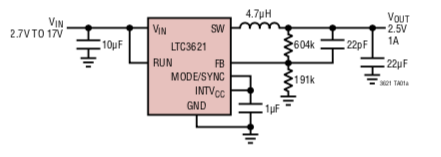
\includegraphics[width=0.6\textwidth]{./img/ltc3621.png}
  \caption{Darstellung des LTC3621 mit beispielhafter Beschaltung gemäß Datenblatt~\cite{ltc3621}}\label{fig.ltc3621}
\end{figure}

Zusätzlich verfügt dieser Regler über die Option, über einen Befehl des Mikrocontrollers manuell ein- bzw. ausgeschaltet zu werden, was weiterhin günstig für den Gesamtstromverbrauch ist.

\subsubsection{3V3}\label{subsubsec.3v3}
Im folgenden soll hauptsächlich auf die Dimensionierung des Spannungsteilers zur Erzeugung von 3,3\,V eingegangen werden. Der Regler hat dabei eine interne Referenzspannung am FB-Pin, die 0,6\,V beträgt, über die die Ausgangsspannung geregelt wird. 

\begin{figure}[H]
  \centering
  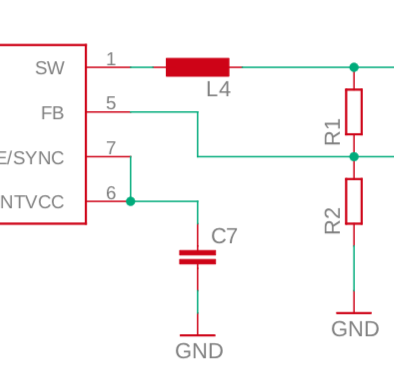
\includegraphics[width=0.4\textwidth]{./img/spannungsteiler_3v3.png}
  \caption{Spannungsteiler am FB-Pins des 3V3 Reglers}\label{fig.spgsteiler3v3}
\end{figure}

Es kann somit der folgende Spannungsteiler aufgestellt werden:

\begin{minipage}{\textwidth}
\begin{equation}\label{eq:Spannungsteiler3v3}
\frac {U_{FB}}{U_a}{=}  \frac{R_{101}}{R_{101}+R_{100}}
\end{equation}
\end{minipage}

Mit $U_{FB}=0,6\,\si{\volt}$, $U_a=3,3\,\si{\volt}$ und $R_{101}=150\,\si{\kilo\ohm}$ ergibt sich:

\begin{minipage}{\textwidth}
\begin{equation}\label{eq:Spannungsteiler3v3b}
\frac {0,6\,\si{\volt}}{3,3\,\si{\volt}}{=}  \frac{150\,\si{\kilo\ohm}}{150\,\si{\kilo\ohm}+R_{100}} \Rightarrow R_{100}=680\,\si{\kilo\ohm}
\end{equation}
\end{minipage}

Der Spannungsteiler wurde hochohmig dimensioniert, um den Stromfluss möglichst klein zu halten.


%Spannungsteiler Formel, was wird alles von 3V3 versorgt 
\subsubsection{5V}\label{subsubsec.5v}
Die Bestimmung des Spannungsteilers für die Erzeugung von 5V erfolgt analog zu Abschnitt \ref{subsubsec.3v3}. Es lässt sich folgender Spannungsteiler aufstellen:

\begin{figure}[H]
  \centering
  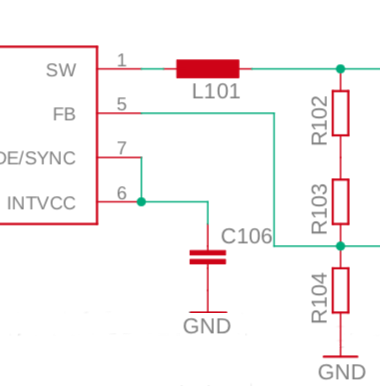
\includegraphics[width=0.4\textwidth]{./img/spannungsteiler_5v.png}
  \caption{Spannungsteiler am FB-Pins des 5V Reglers}\label{fig.spgsteiler5v}
\end{figure}

Dieser wird beschrieben durch:

\begin{minipage}{\textwidth}
\begin{equation}\label{eq:Spannungsteiler5v}
\frac {U_{FB}}{U_a}{=}  \frac{R_{104}}{R_{104}+R_{103}+R_{102}}
\end{equation}
\end{minipage}

Mit $U_{FB}=0,6\,\si{\volt}$, $U_a=3,3\,\si{\volt}$ und $R_{104}=100\,\si{\kilo\ohm}$ ergibt sich:

\begin{minipage}{\textwidth}
\begin{equation}\label{eq:Spannungsteiler5vb}
\frac {0,6\,\si{\volt}}{3,3\,\si{\volt}}{=}  \frac{100\,\si{\kilo\ohm}}{10\,\si{\kilo\ohm}+R_{103}+R_{102}} \Rightarrow R_{103}=680\,\si{\kilo\ohm}; R_{102}=47\,\si{\kilo\ohm}
\end{equation}
\end{minipage}



\subsection{Spannungsabschaltung}\label{subsec.Spannungsabschaltung}
Im Zuge der Überlegungen bezüglich möglicher Energiesparmaßnahmen wurden sowohl das Bluetooth- als auch das GPS-Modul als große Verbraucher ermittelt. Da beide Module auch nicht dauerhaft benötigt werden -- das GPS-Modul nur alle 15 Minuten zur Neuausrichtung des Panels und das Bluetooth-Modul nur nach Bedarf -- ist es sinnvoll, die Betriebsspannungen beider Module schaltbar zu machen. Eine Möglichkeit dafür ist die Verwendung eines p-Kanal-Mosfets, der von einem n-Kanal-Mosfet getrieben wird. Diese Schaltung wird in Abbildung \ref{fig.spgsabschaltung} dargestellt.

\begin{figure}[H]
  \centering
  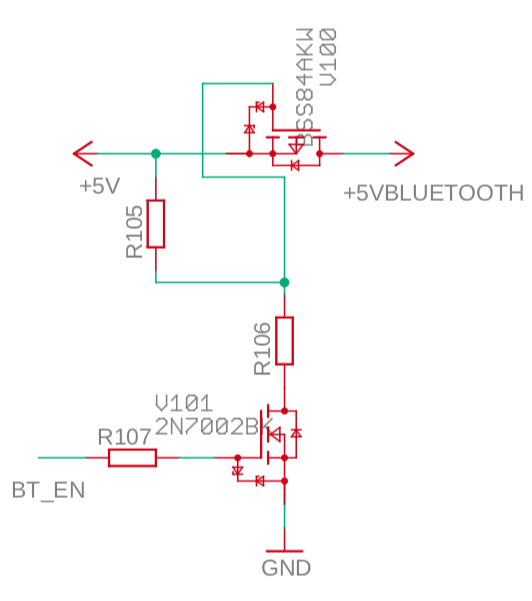
\includegraphics[width=0.4\textwidth]{./img/spannungsabschaltung.png}
  \caption{Spannngsabschaltung Bluetooth-Modul}\label{fig.spgsabschaltung}
\end{figure}

Bei einem Einschaltsignal über BT\_EN vom Mikrocontroller schaltet der n-Kanal-Mosfet V101 durch; der Spannungsteiler aus $R_{105}$ und $R_{106}$ ist aktiv. Es sei $R_{105}=100\,\si{\kilo\ohm}$ und $R_{106}=1\,\si{\kilo\ohm}$. Daraus ergibt sich für die Gate-Source-Spannung des p-Kanal-Transistors $U_{GS}$:

\begin{minipage}{\textwidth}
\begin{equation}\label{eq:UGS}
{U_{GS}}{=} 5\,\si{\volt}-5\,\si{\volt}\cdot \frac{1\,\si{\kilo\ohm}}{101\,\si{\kilo\ohm}}{=}4,95\,V
\end{equation}
\end{minipage}

Damit schaltet der p-Kanal-Transistor mit $U_{GS,th}=1,6\,V$ sicher durch.
Die Schaltung für das GPS-Modul wird analog dazu entworfen.


\subsection{Messung Strom/Spannung}\label{subsec.MessungStromSpannung}
Aus den Anforderungen abgeleitet wird auf der Platine die Messung von Strom und Spannung implementiert. Für die Messung der Stromaufnahme werden zwei Stromsensoren vom Typ ACS172 verwendet. Diese messen den Ladestrom der Batterie und die Stromaufnahme des Boards und geben diese Werte an den Mikrocontroller.
Die Spannungsmessung wird mit einem einfachen Spannungsteiler umgesetzt, sodass bei $U_{Bat}=12\,\si{\volt}$ 3,3\,V nicht überschritten werden. Mit $R_{109}=270\,\si{\kilo\ohm}$ und $R_{110}=100\,\si{\kilo\ohm}$ ergibt sich eine maximale Spannung von 3,24\,V.






\section{Kompassmodul}

Als Kompass dient uns der Sensor XYZ von der Firma ASDF. Verwendet wird er, um die Ausrichtung der Wetterstation zu messen. Diese Information wird benötigt, um das Solarpanel korrekt zur Sonne auszurichten. Die Ausrichtung wird in Kapitel (Referenz zu Kapitel solartracking) genauer beschrieben.

Bild Sensor

Wichtige Kenndaten blabla

Stromaufnahme

\subsection{C-Code}

Der Sensor wird über eine I²C Schnittstellen angesprochen. Er liefert seine Daten folgendermaßen...

Sleepmode, Forcemode

\section{GPS}

\subsection{C-Code}

\section{Anemometer}

Viel gut als alte, voll simpel, much wow

\subsection{C-Code}

\section{Neigungssensor}

\subsection{C-Code}

\section{Beliebeiger anderer Sensor}

\subsection{C-Code}

\subsection{C-Code}

\section{Ausrichtung des Solarpanels}\label{sec:ausrichtung des Solarpanels}
Um die Leistungsaufnahme des Solarpanels zu optimieren ist es notwendig dieses direkt auf die Sonne auszurichten und diese Ausrichtung auch in geeigneten Zeitabständen zu korrigieren. Im Vergleich mit einem fest ausgerichteten Solarpanel konnten J. Rizek \emph{et al.} mit einem nachgeführten Solarpanel beispielsweise die Leistungsaufnahme um durchschnittlich 30\% erhöhen~\cite{Rizek2008}.

Hierfür kommen grundsätzlich verschiedene Methoden in Frage. In diesen Fall soll die Position der Sonne relativ zur Wetterstation auf Grundlage des Längen- und Breitengrades, der Uhrzeit und des Kalendertages berechnet werden. Diese Information werden über das GPS-Modul bereitgestellt. Anschließend wird das Solarpanel mit Hilfe der Motoren, des Kompass-Moduls und des, am Panel befestigten Neigungssensors, auf die Sonne ausgerichtet.

\subsection{Berechnung der Sonnenposition}\label{sec:berechnung_der_sonnenposition}
Da die Formeln zur Berechnung der Sonnenposition in diesem Projekt lediglich benutzt werden wird an dieser Stelle auf eine Herleitung verzichtet. Die verwendeten Formeln können beispielsweise im \emph{Astronomical Almanac}~\cite{Anon1984} gefunden werden. \emph{M. L. Roderick} beschreibt die nötigen Berechnungen in seinem Report~\cite{Roderick1992} und liefert zudem compilierbaren C-Code. Dieser wird im folgenden zur Berechnung der Sonnenposition verwendet.

Die Position der Sonne im Bezug auf einen Beobachter auf der Erde lässt sich durch die Werte \emph{Zenith} und \emph{Azimut} eindeutig beschreiben. Der Zenith beschreibt den Winkel zwischen einer Linie vom Beobachter zur Sonne und der Vertikalen. Der Azimut den Winkel zwischen der Horizontalen und Norden. Dabei stehen beispielsweise ein Azimut von \SI{90}{\degree} für Osten, \SI{180}{\degree} für Süden und \SI{270}{\degree} für Westen. Eine Veranschaulichung kann in Abbildung~\ref{fig:zen_azi} gefunden werden.

\begin{figure}[H]
  \centering
  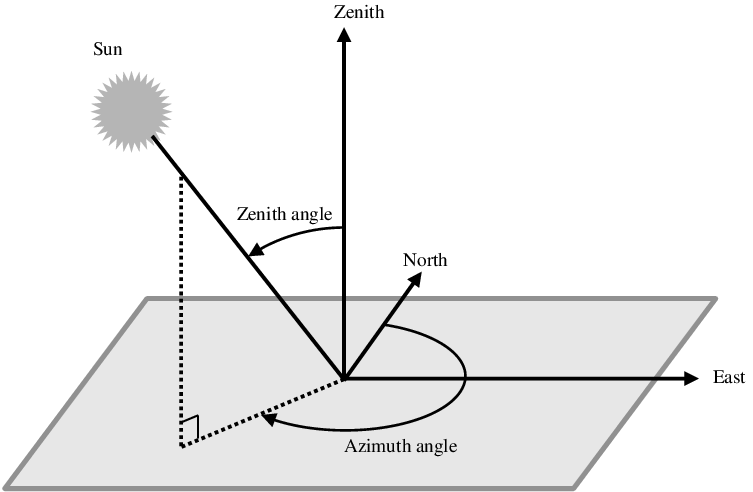
\includegraphics[width=\textwidth]{./img/Representation-of-azimuth-and-zenith-angles.png}
  \caption{Beschreibung der Sonnenposition durch Zenith und Azimut~\cite{Nou2016}}\label{fig:zen_azi}
\end{figure}

Die Genauigkeit der verwendeten Formeln beträgt laut dem \emph{Astronomical Almanac} 


%%% Local Variables:
%%% mode: latex
%%% TeX-master: "../termpaper"
%%% End:

\section{Benutzeroberfläche}\label{sec:benutzeroberflaeche}
Um eine leichte Handhabung der Wetterstation zu ermöglichen wird eine, auf dem PyQt5~\cite{pyqt5} Framework basierende, Benutzeroberfläche verwendet. Für die Kommunikation mit der Wetterstation muss der Computer über eine Bluetooth-Schnittstelle verfügen

In diesem Kapitel wird die zur Verfügung stehenden Funktionen sowie die Entwicklung der Benutzeroberfläche beschrieben.

\subsection{Funktionen}\label{sec:bo_funktionen}
Die Benutzeroberfläche (s. Abb.~\ref{fig:ui_open}) verfügt über zwei Hauptansichten: eine graphische (s. Abb.~\ref{fig:ui_graph}) und eine tabelarische (s. Abb.~\ref{fig:ui_table}).

Diese unterscheiden sich jeweils nur durch die Anzeigevariante (s. Abb.~\ref{fig:ui_open} und~\ref{fig:ui_table} (1)).

Über das Konsolenfenster (s. Abb.~\ref{fig:ui_graph} (2)) können die im Kapitel (HIER KAPITELLINK EINFÜGEN) beschrieben AT-Befehle an die Wetterstation gesendet werden. Sowohl die gesendeten als auch die empfangenen Daten werden im Konsolenfenster angezeigt. Über die Schaltfläche \emph{Clear} lässt sich der Inhalt des Konsolenfensters löschen. Die Größe des Konsolenfensters und des Anzeigefensters kann beliebig verändert werden.

Das Menü (s. Abb.~\ref{fig:ui_graph} (3)) enthält die zur Bedienung notwendigen Befehle. Es sind nicht alle AT-Befehle implementiert. Die AT-Befehle, welche nicht implementiert sind können manuell über das Konsolenfenster an die Wetterstation gesendet werden. Einige der Menübefehle wurden aufgrund von Zeitmangel nicht implementiert und sind daher ausgegraut. Das Menü enthällt die Folgenden Befehle:
\begin{itemize}
\item File
  \begin{itemize}
  \item Save (nicht implementiert): Speichert die empfangenen Daten in einer CSV-Datei ab.
  \item Open (nicht implementiert): Lädt die Daten aus einer CSV-Datei in das Programm.
  \end{itemize}
\item Control
  \begin{itemize}
  \item Set Time
    \begin{itemize}
    \item UTC: Setzt die Uhrzeit und das Datum der Wetterstaion auf die Koordinierte Weltzeit. Die Uhrzeit wird der Computeruhr entnommen.
    \item Custom (nicht implementiert): Öffnet ein Fenster in welches eine beliebige Uhrzeit und Datum eingegeben werden kann. Diese wird anschließend auf die Wetterstaion gespielt.
    \end{itemize}
  \item Set Position
    \begin{itemize}
    \item Hamburg: Setzt die Postition der Wetterstation auf (53.556354, 10.022650) (HAW Hamburg).
    \item Custom (nicht implementiert): Öffnet ein Fenster in welches beliebige Koordination eingegeben werden können. Diese werden anschließend auf die Wetterstation übertragen.
    \end{itemize}
  \item Adjust Orientation (nicht implementiert): Gibt der Wetterstation den Befehl sich sofort neu auszurichten.
  \item Set Update-Interval: Bestimmt das Interval, in welchem eine Verbindung mit der Wetterstaion aufgebaut wird. Nach dem Aufbau der Verbindung werden die neuen Messdaten angefordert, empfangen und dargestellt. Anschließend wird die Verbindung, zwecks Energiespaaren, wieder geschloßen.
    \begin{itemize}
    \item 5 sec: fünf Sekunden
    \item 1 min: eine Minute
    \item 15 min: fünfzehn Minuten
    \item 1 h: eine Stunde
    \item Manuel: Kein Automatisches Anfordern der Messdaten. Zum Anfordern der Messdaten muss die \emph{Update}-Schaltfläche betätigt werden.
    \end{itemize}
  \item Set Measuring-Interval: Schickt einen Befehl an die Wetterstation, welcher vorgibt in welchem Interval Messungen durchzuführen sind.
    \begin{itemize}
    \item 5 sec: fünf Sekunden
    \item 15 sec: fünfzehn Sekunden
    \item 1 min: eine Minute
    \end{itemize}
  \end{itemize}
  \begin{itemize}
  \item View: Bestimmt das Zeitinterval, welchen in der graphischen Anzeige dargestellt wird.
    \begin{itemize}
    \item Last Minute: letzte Minute
    \item Last 15 Minutes: letzten fünfzehn Minten
    \item Last Hour: letzte Stunde
    \item Last Day: letzter Tag
    \item Last Week: letzte Woche
    \item Last Month: letzter Monat
    \item Custom (nicht implementiert): Der dagestellt bereich wird über die Elemente zur Darstellund der Start- und Stopzeit (s. Abb.~\ref{fig:ui_graph} (4)) eingestellt. Der Bereich wird im gegensatz zu den anderen Optionen nicht automatisch mit voranschreiten der Zeit geupdatet.
    \end{itemize}
  \end{itemize}
\item Mode:
  \begin{itemize}
  \item Enable Debug: Aktiviert den Debug-Modus. Debugnachrichten werden angezeigt.
  \item Disable Debug: Deaktiviert den Debug-Modus. Debugnachrichten werden nicht angezeigt.
  \item Enable Com: Baut manuell eine Bluetooth-Verbindung zur Wetterstation auf. Dies ist notwendig, wenn Befehle zur Wetterstaition gesendet werden sollen. Für das automatische, periodische Einlesen der Messdaten ist dies nicht notwendig. Es gibt momentan keine möglichkeit den für die Verbindung verwendeten Com-Port über die Benutzeroberfläche anzupassen. Stattdessen muss dieser manuell in der Datei \emph{main\_ctrl.py} geändert werden.
  \item Disbale Com: Schließt die Bluetooth-Verbindung zur Wetterstaion.
  \end{itemize}
\end{itemize}

Die Anzeigen (4) (s. Abb.~\ref{fig:ui_graph}) zeigen, wie bereits erwähnt, das Interval an, welches dargestellt wird. Ist dieses Interval nicht auf \emph{Custom} gestellt, so ist die Endzeit immer die aktuelle Zeit. Die Startzeit ergibt entsprechnd des eingestellen Zeitintervalls.

Über die Schaltfächen (5) (s. Abb.~\ref{fig:ui_graph}) können zwei Messkurven aufgewählt werden, welche dargestellt werden sollen. Die Schaltfläche \emph{Update} ist für das manuelle Anfordern der Messdaten notwendig. Unter den Schaltflächen werden die, über das Fadenkreuz (6) (s. Abb.~\ref{fig:ui_graph}) ausgewählten, Messpunkte schriftlich dargestellt.
\begin{figure}[H]
  \centering
  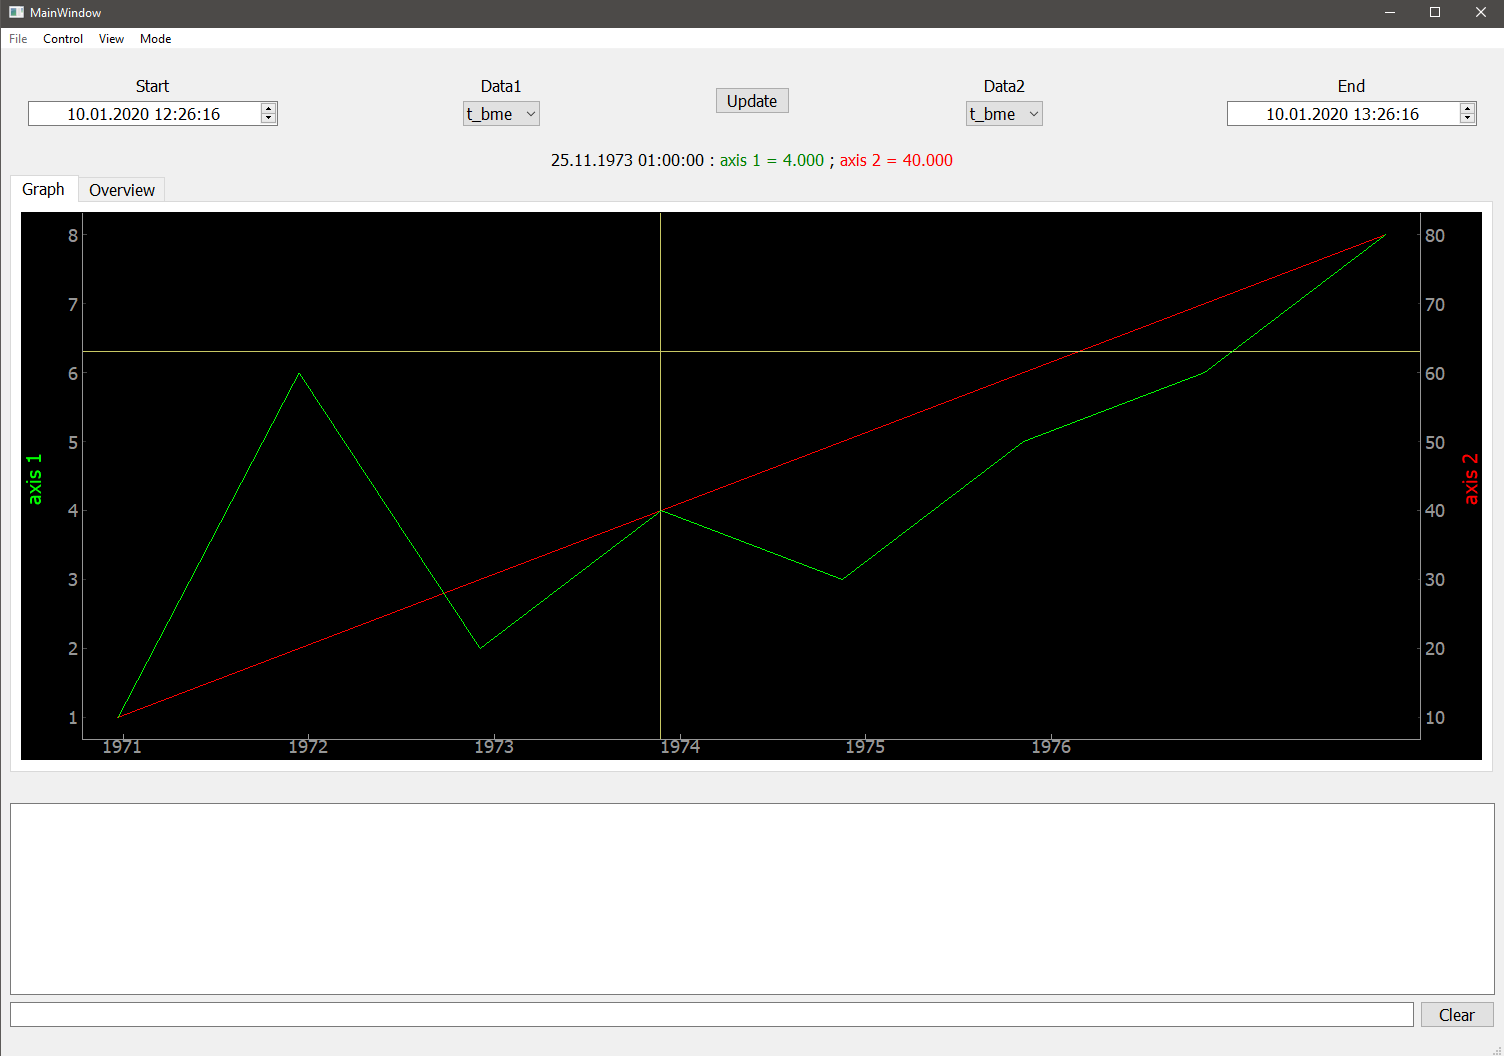
\includegraphics[width=\textwidth]{./img/ui_open}
  \caption{Benutzeroberfläche nach dem offnen. Dagestellt sind zwei vordefinierte Testkurven, welche nach Empfang des ersten Messwertes gelöscht werden.}\label{fig:ui_open}
\end{figure}
\begin{figure}[H]
  \centering
  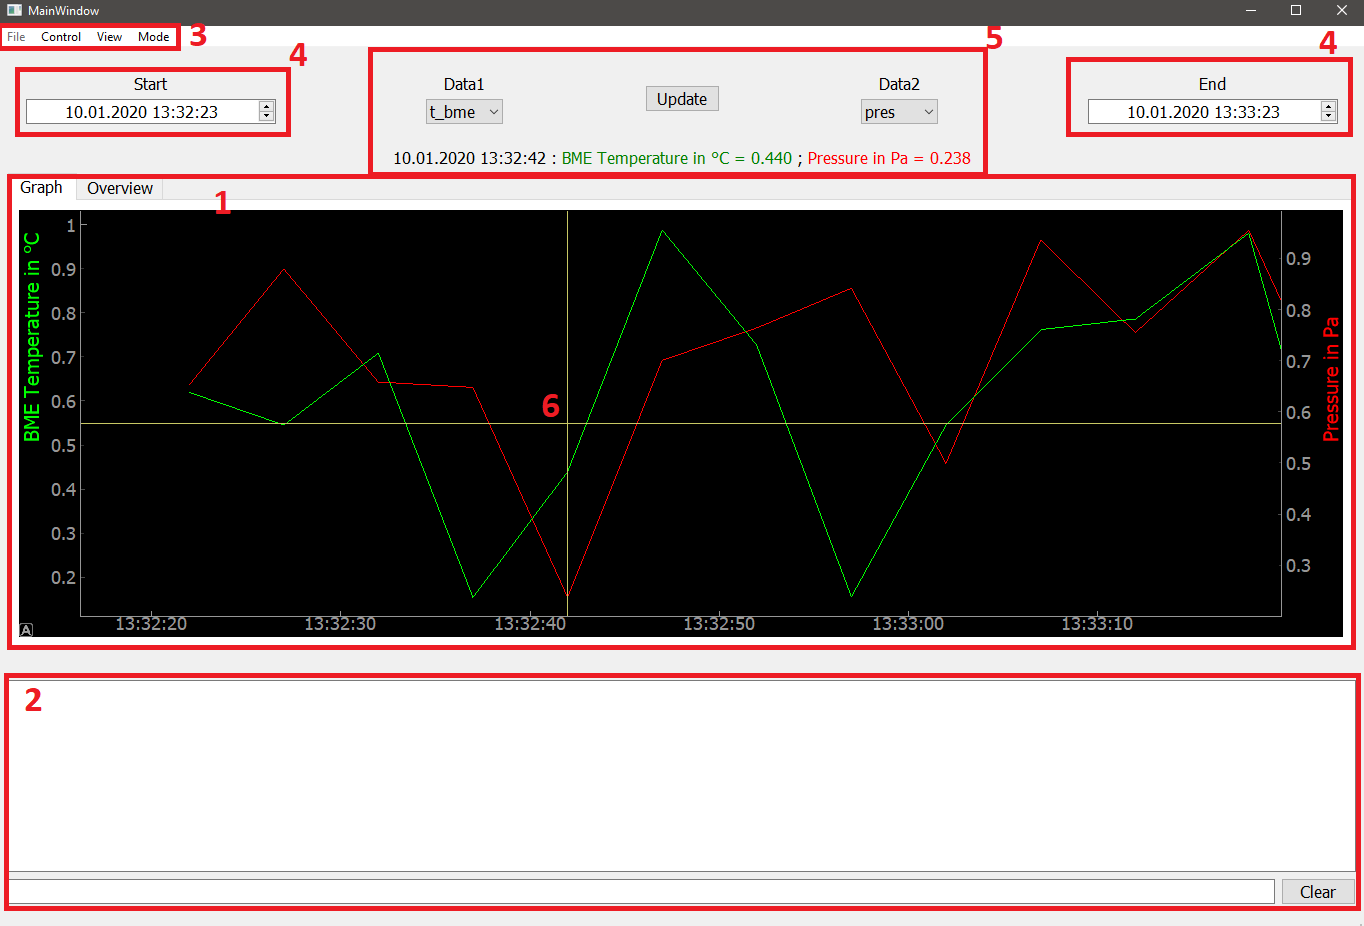
\includegraphics[width=\textwidth]{./img/ui_simulated_graph}
  \caption{Benutzeroberfläche: (1) Graphische Darstellung der Messwerte. (2) Konsolenfenster. (3) Kontrollmenü mit den wichtigsten Befehlen. (4) Start- und Endzeit der graphischen Darstellung. (5) Auswahl der dargestellten Messwerte, Schaltfläche zum manuellen Updaten der Messwerte und Anzeige der Messwerte an der aktuellen Fadenkreuzposition. (6) Fadenkreuz zum Anzeigen spezifischer Messwerte.}\label{fig:ui_graph}
\end{figure}
\begin{figure}[H]
  \centering
  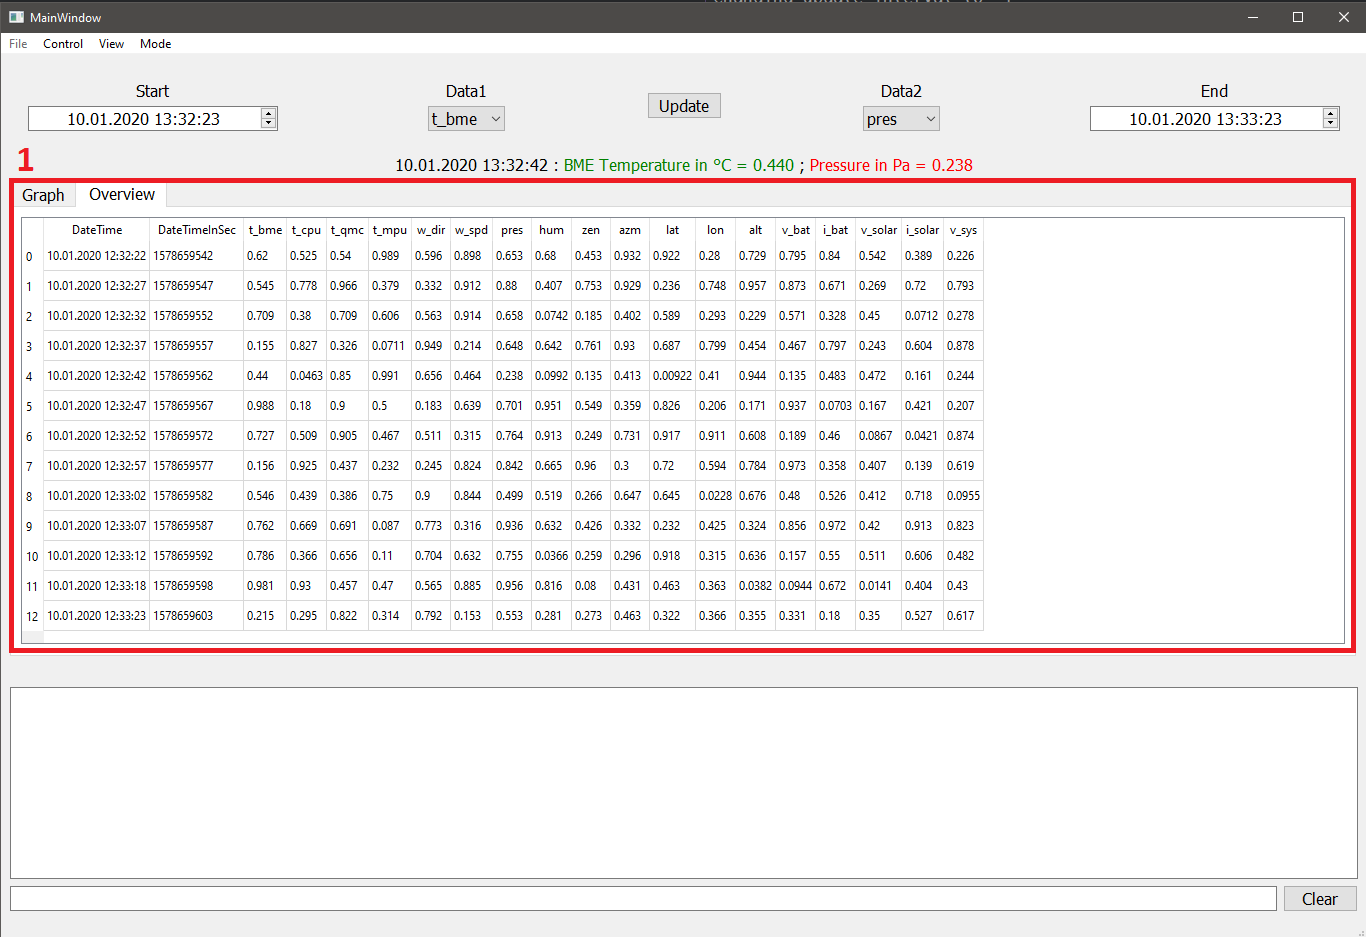
\includegraphics[width=\textwidth]{./img/ui_simulated_table}
  \caption{Benutzeroberfläche: (1) Tabelarische Darstellung von simulierten Werten.}\label{fig:ui_table}
\end{figure}

\subsection{Entwicklung}\label{sec:bo_entwicklung}
In diesem Kapitel werden die, für die Benutzeroberfläche implementierten Funktionen, \emph{nicht} im Detail beschrieben. Es soll lediglich ein Überblick über die Verwendeten Technologien und den Aufbau der Projekts gegeben werden. Bei der Entwicklung wurde versucht der Code in einer Art und Weise zu schreiben, welche es anderen Personen ermöglicht ohne eine ausführliche Beschreibung des gesammten Codes, an diesem weiterzuarbeiten.

Als Entwicklungssprache wurde Python 3 verwendet. Der verwendete Quellcode befindet sich im Ordner \textrm{UI}. Die Oberfläche wurde nach dem Model-View-Controller Design-Muster (s. z.B.~\cite{deacon09}) entwickelt. Für einige der Funktionalitäten wurde Code aus den, im PyQt5-Package enthaltenen, Beispielen als Vorlage verwendet. 


%%% Local Variables:
%%% mode: latex
%%% TeX-master: "../termpaper"
%%% End:

\section{3D gedruckte Komponenten}\label{sec:gehaeuse}
Für das Unterbringen des Mikroprozessors und der Sensoren werden zwei verschiedene Gehäusevarianten verwendet. Dieses Kapitel beschäfftigt sich mit deren Entwurf, sowie dem Entwurf des Adapters, mit welchem die Windfahne und das Anemometer an der Wetterstation befestigt sind.

Für den Entwurf der Komponenten wurde die Studentenversion von Autocad Fusion 360 verwendet.

\subsection{Hauptgehäuse}\label{sec:ge_haupt}
Das Hauptgehäuse beinhaltet das Mikroprozessor-Board mit den zwei aufsteckbaren Platinen sowie den Sensoren. Drei der Sensoren befinden sich nicht im Hauptgehäuse (s. Kap.~\ref{sec:ge_neben}).

Das Gehäuse besteht aus zwei Teilen (s. Abb. \ref{fig:main}), dem Hauptteil (links) und dem Deckel (rechts). Das STM8 Nucleo Board wird von drei Pins in Position gehalten (s. Abb.~\ref{fig:main},~\ref{fig:main_top}). In der Vorderseite befinden sich zwei Aussparungen (s. Abb.~\ref{fig:main_front}). Über die Linke ist der USB-Port des Mikroprozessor-Boards erreichbar. Hinter der Rechten befindet sich der Motortreiber, welcher auf einer leicht erhöhten Plattform plaziert wird (s. Abb.~\ref{fig:main_top}). Über die Aussparung an der rechten Seite kann die SD-Karte erreicht werden. Die Aussparung an der hinteren Seite wird verwendet, um alle externen Komponenten mit dem Mikroprozessor-Board zu verbinden.

Im Deckel befinden sich drei Löcher, in welche Status-LEDs untergebracht werden.

Das Hauptteil und der Deckel werden lediglich aufeinander gesteckt. Bedingt durch die Geometrie entsteht ein relativ fester Halt. Optional können die Komponenten über die vier Aussparungen an den Seiten, mit beispielsweise Kabelbindern, zusätzlich gesichert werden.
\begin{figure}[H]
  \centering
  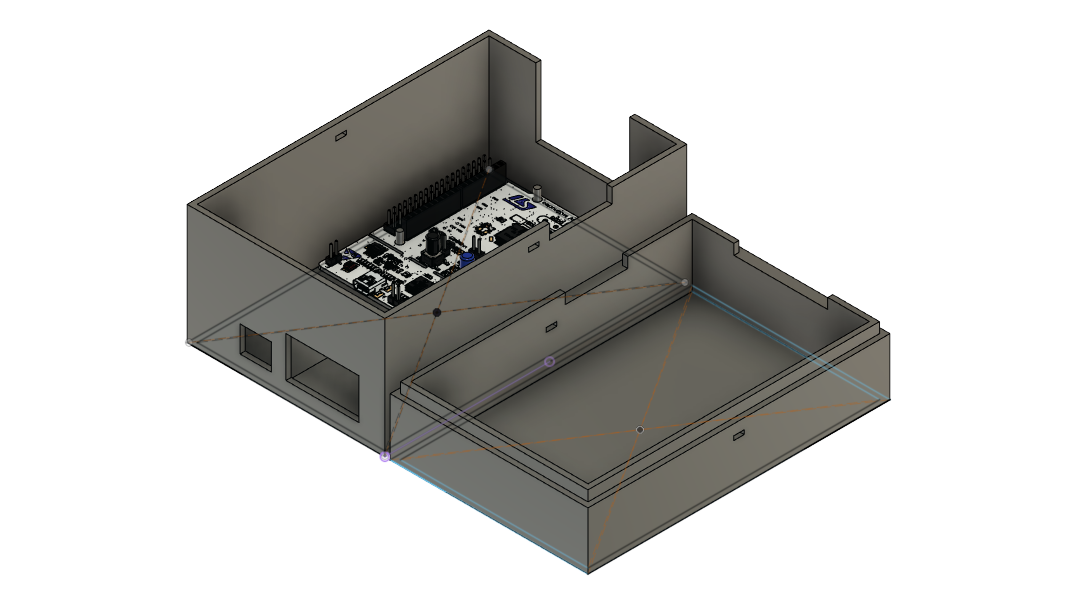
\includegraphics[width=\textwidth]{./img/ST_MainBodyv13}
  \caption{Hauptgehäuse}\label{fig:main}
\end{figure}
\begin{figure}[H]
  \centering
  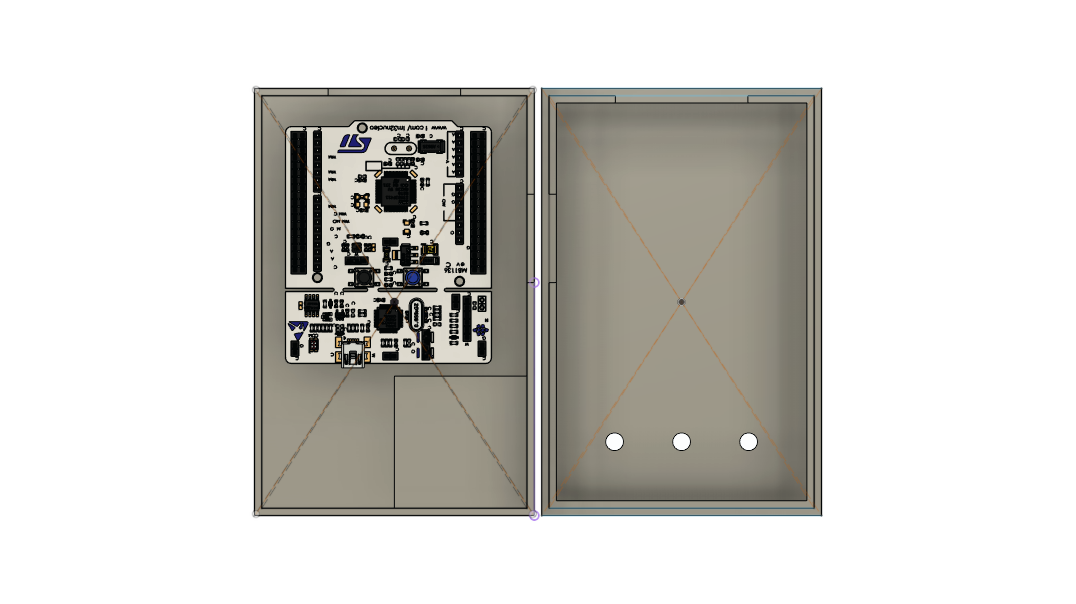
\includegraphics[width=\textwidth]{./img/ST_MainBodyv13_top}
  \caption{Hauptgehäuse, Ansicht von oben}\label{fig:main_top}
\end{figure}
\begin{figure}[H]
  \centering
  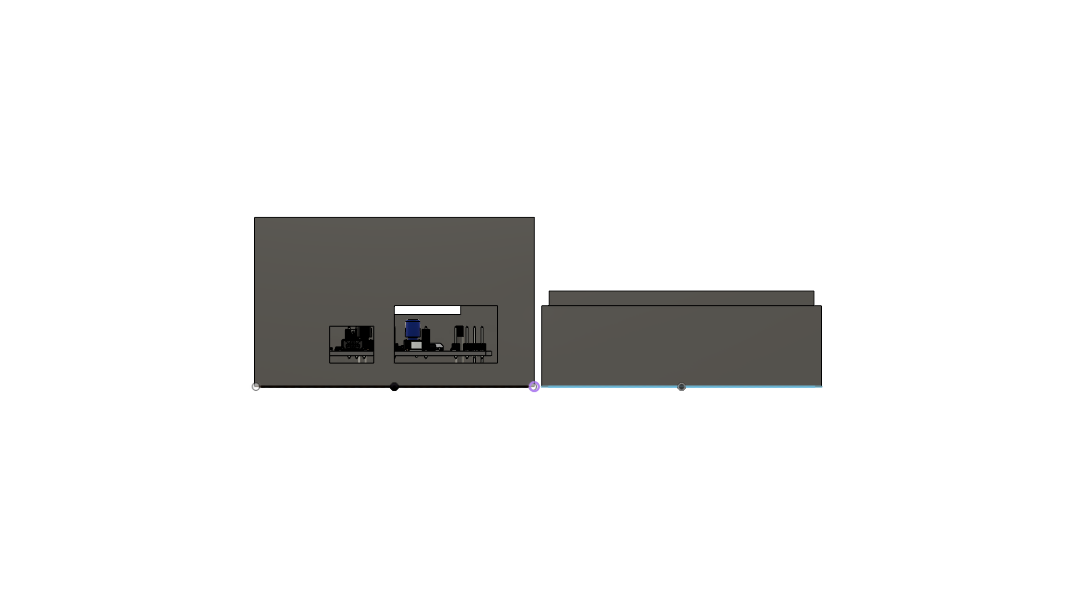
\includegraphics[width=\textwidth]{./img/ST_MainBodyv13_front}
  \caption{Hauptgehäuse, Ansicht von vorne}\label{fig:main_front}
\end{figure}
\subsection{Nebengehäuse}\label{sec:ge_neben}
Es wird jeweils ein Nebengehäuse für folgende Sensoren verwendet:
\begin{itemize}
\item der Neigungssensor, welcher an der Rückseite des Solarpanels befestigt werden muss,
\item der GPS-Empfänger, welcher für besseren Empfang am oberen Ende der Wetterstation befestigt wird,
\item das Kompass-Modul, welches empfindlich auf elektro-magnetische Störungen reagiert und aus diesem Grund auch am oberen Ende der Wetterstation untergebracht wird (auf der Seite gegenüber des GPS-Empfängers).
\end{itemize}
Die Nebengehäuse bestehen aus zwei Teilen, welche aufeinandergesteckt werden und zusätzlich, optional, mittels Kabelbinder gesichert werden (s. Abb.~\ref{fig:secondary},~\ref{fig:secondary_front}).

Die Nebengehäuse werden mit einer Schraube und einer Mutter am Aluminium-Profil der Wetterstation befestigt (s.Abb.~\ref{fig:secondary_top}). Das Nebengehäuse, welches sich auf dem Solarpanel befindet, kann nicht geschraubt werden und wird entsprechend mit Klebstoff befestigt.

Die runden Aussparungen an der linken und rechten Seiten dienen dem Durchführen von benötigten Leitungen.
\begin{figure}[H]
  \centering
  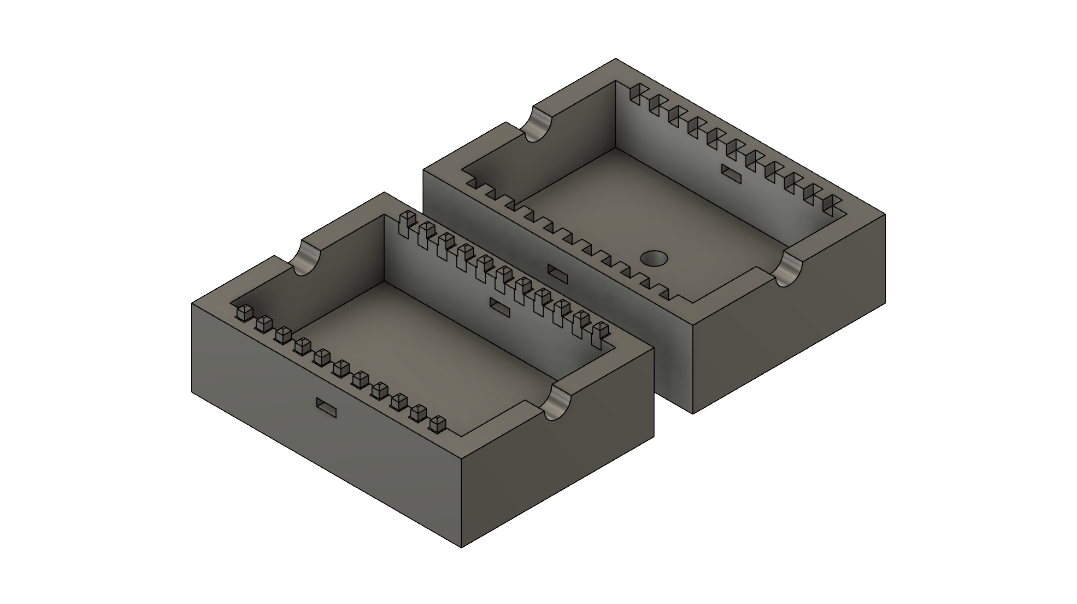
\includegraphics[width=\textwidth]{./img/ST_Halterv5}
  \caption{Nebengehäuse}\label{fig:secondary}
\end{figure}
\begin{figure}[H]
  \centering
  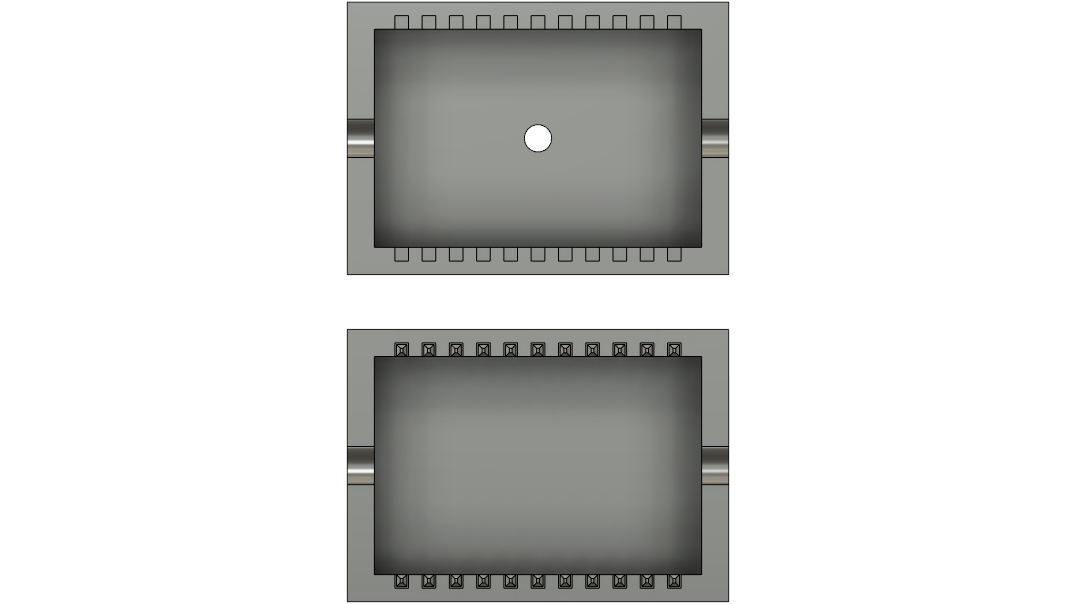
\includegraphics[width=\textwidth]{./img/ST_Halterv5_top}
  \caption{Nebengehäuse, Ansicht von oben}\label{fig:secondary_top}
\end{figure}
\begin{figure}[H]
  \centering
  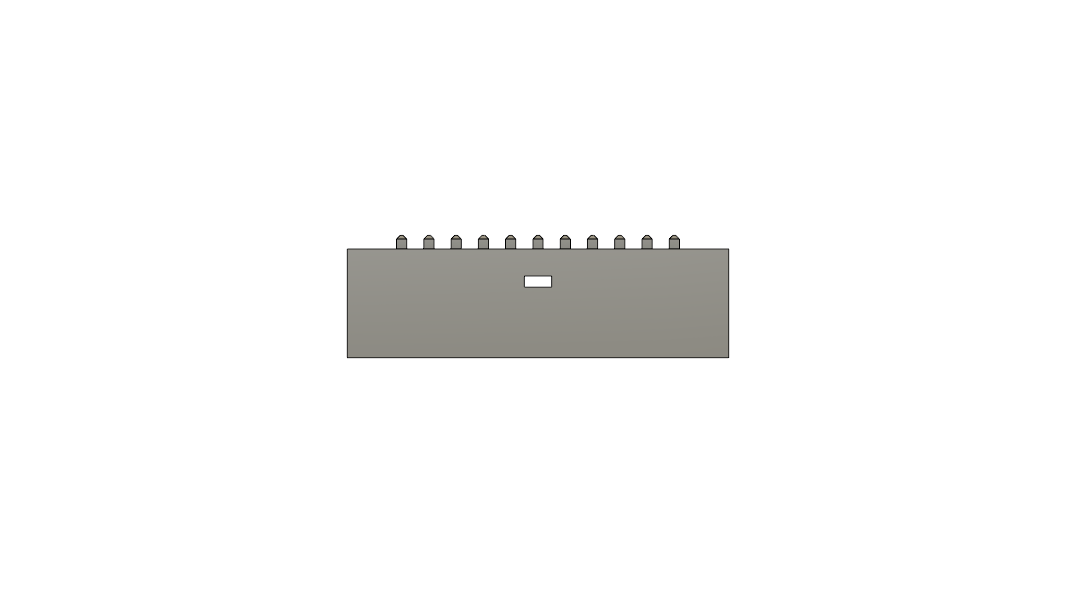
\includegraphics[width=\textwidth]{./img/ST_Halterv5_front}
  \caption{Nebengehäuse, Ansicht von vorne}\label{fig:secondary_front}
\end{figure}
\subsection{Adapter}\label{sec:ge_adapt}
Der Adapter wird verwendet, um eine feste Verbindung zwischem dem Alluminium-Profil der Wetterstaion und dem Mast mit Windfahne und Anemometer herzustellen.

Die Verbindung zur Wetterstation erfolgt durch Stecken der vier trapez-förmigen Steckkontakte am unteren Ende des Adapters (s. Abb.~\ref{fig:adapter},~\ref{fig:adapter_front}).

Der Mast wird von oben auf die angepasste Aussparung gesteckt. Optional kann dieser mittels Schraubverbindung fixiert werden (s. Abb.~\ref{fig:adapter},~\ref{fig:adapter_top}).
\begin{figure}[H]
  \centering
  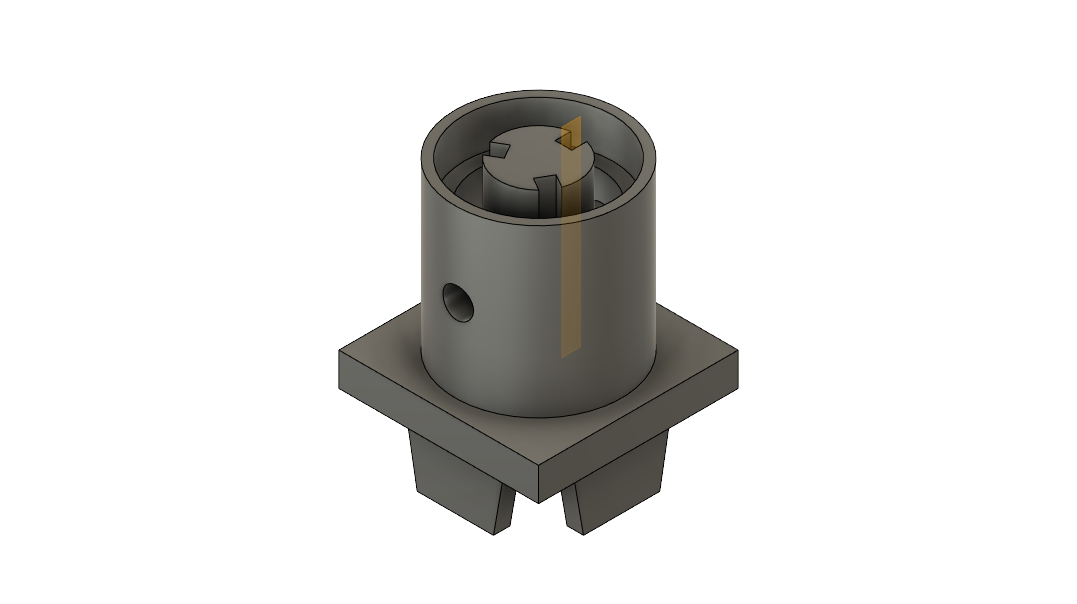
\includegraphics[width=\textwidth]{./img/ST_Adapterv4}
  \caption{Adapter}\label{fig:adapter}
\end{figure}
\begin{figure}[H]
  \centering
  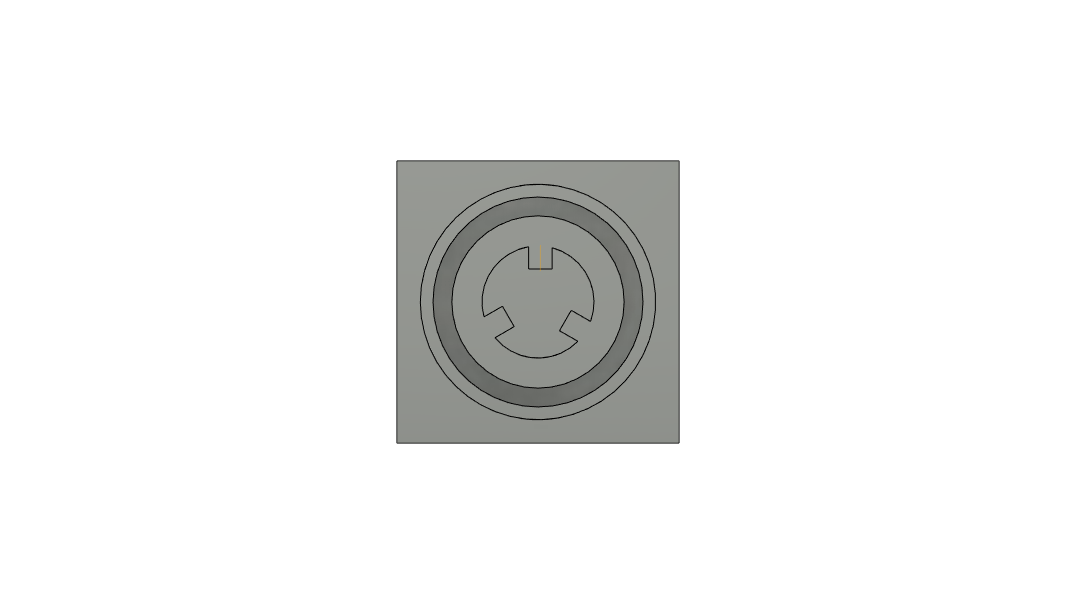
\includegraphics[width=\textwidth]{./img/ST_Adapterv4_top}
  \caption{Adapter, Ansicht von oben}\label{fig:adapter_top}
\end{figure}
\begin{figure}[H]
  \centering
  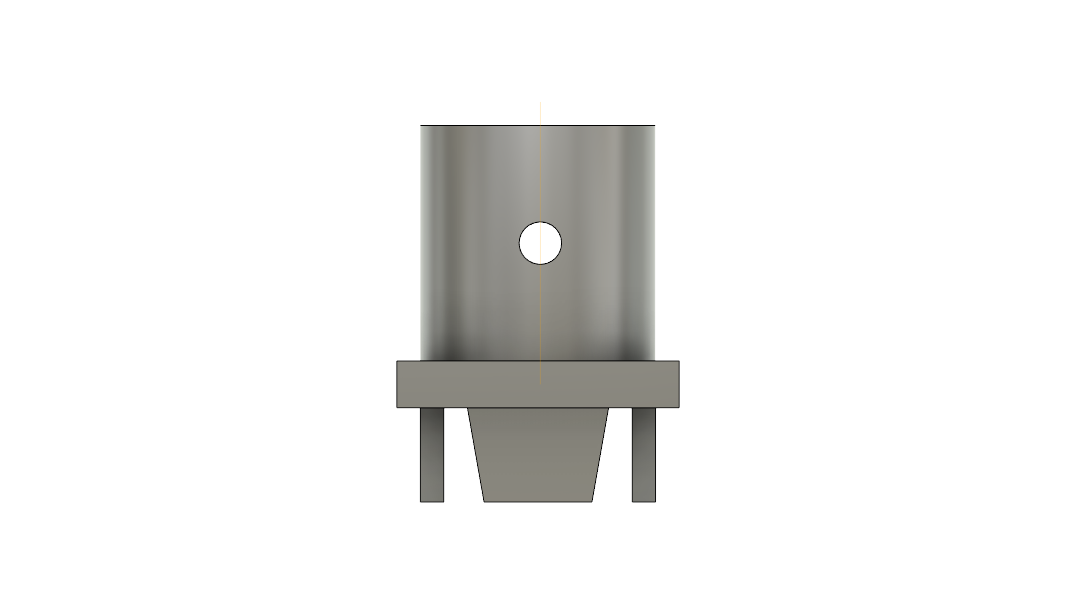
\includegraphics[width=\textwidth]{./img/ST_Adapterv4_front}
  \caption{Adapter, Ansicht von vorne}\label{fig:adapter_front}
\end{figure}
\subsection{Herstellung}\label{sec:ge_herst}
Alle Komponenten wurden in PLA mit einer Schichtdicke von \SI{0.2}{\milli\meter} gedruckt. Es wurden zwei bis drei Top-, Buttom- und Wandschichten gedruckt. Da die Komponenten keine großen Kräfte aushalten müssen wurden sie lediglich mit einem Infill von \SI{10}{\percent} bis \SI{20}{\percent} gedruckt.
%%% Local Variables:
%%% mode: latex
%%% TeX-master: "../termpaper"
%%% End:

%\bibliographystyle{plain}
\bibliographystyle{dinat}
\bibliography{literature}

%\Istatement

\end{document}

%%% Local Variables:
%%% mode: latex
%%% TeX-master: t
%%% End:
